
\chapter{Semantics}
\begin{chapquote}{H.G. Rice [1953], \textit{paraphrased by Anders Moller}}
  ``Everything interesting about the behaviour of programs is
  undecidable.''
\end{chapquote}

The goal of \textit{static program analysis} is to verify certain
\textsl{properties} (or \textsl{behaviours}, or
\textsl{specifications}, or \textsl{statements}, ...) of the target
program \textbf{without its execution}.

For program \textsl{P} and property \textsl{S},

\begin{itemize}
\item $ \SEM{P} $: Formal semantics of program \textsl{P}.

\item \textsl{S}: Semantic properties that we're interested in. This
  could be defined in various level, such as ``Division-by-zero will
  \textbf{never} occur'' or ``The variable \textit{i} is always 3''.

\item Soundness: $ analysis(P) = true \implies S $

\item Completeness: $ S \implies analysis(P) = true $

\item Scalability: Time complexity.
\end{itemize}


\textbf{No analysis} can be sound and complete at the same time. If an
analysis is sound, then it is also incomplete, and vice versa.


\section{Soundness}

It is called \textbf{sound} if an analysis for program \textsl{P} says
that it satisfies property \textsl{S}, then the program will truly
satisfy that property.

\textbf{Sound} but \textbf{incomplete} analysis have \textbf{false
  positive}. In other words, it does \textbf{not prove} programs that
satisfy the property.

\begin{figure}[h]
  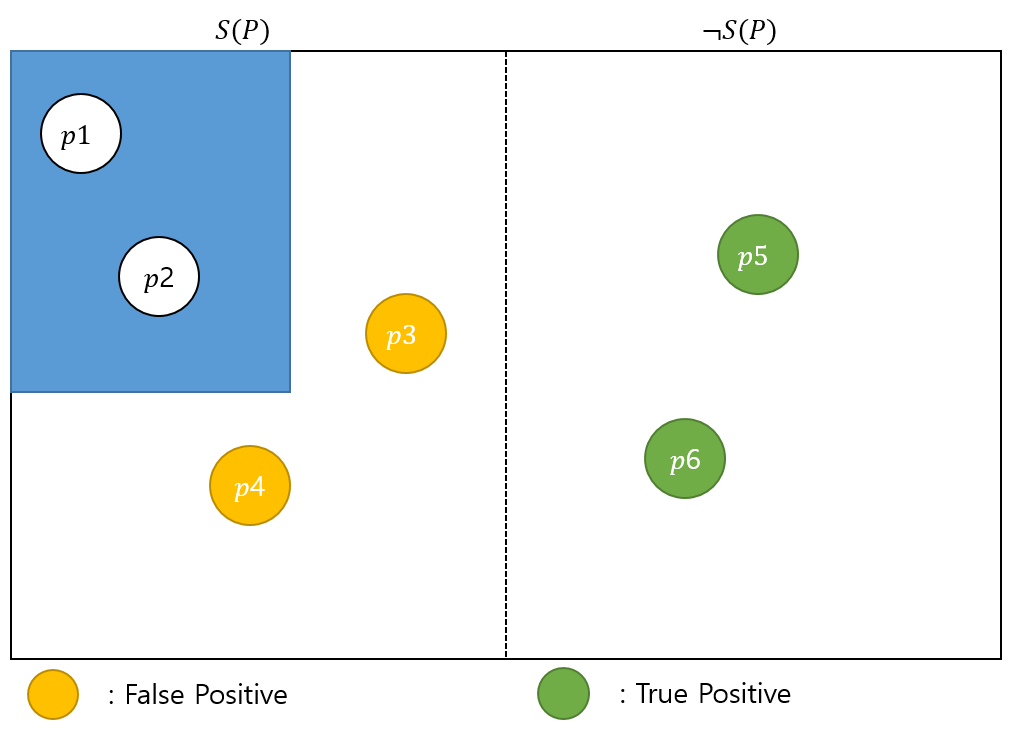
\includegraphics[width=\textwidth]{sound}
  \caption{Sound Analysis}
  \label{fig:sound}
\end{figure}

Figure \ref{fig:sound} shows a sound analysis (the blue area). It
proves correctly for the programs $ p_1 $ and $ p_2 $ that satisfy the
specification ($S(P)$). However, since this analysis is
\textit{incomplete}, it has \textbf{false positives}: it \textbf{does
  not prove} for programs $ p_3 $ and $ p_4 $ that satisfy $S$. In
other words, it proves that $ p_3 $ and $ p_4 $ satisfy $ \neg S(P) $
by emiting \textbf{alarms}, even though they are actually satisfy
$ S(P) $. False positives are also called as \textbf{false alarms}.


\section{Completeness}

An analysis is called \textbf{complete} when a program satisfies a
property \textsl{S}, the analysis for that program says that it will
satisfy that property.


\textbf{Complete} but \textbf{unsound} analysis have \textbf{false
  negative}. In other words, it \textbf{wrongly proves} programs that
does not satisfy the property.


\begin{figure}[h]
  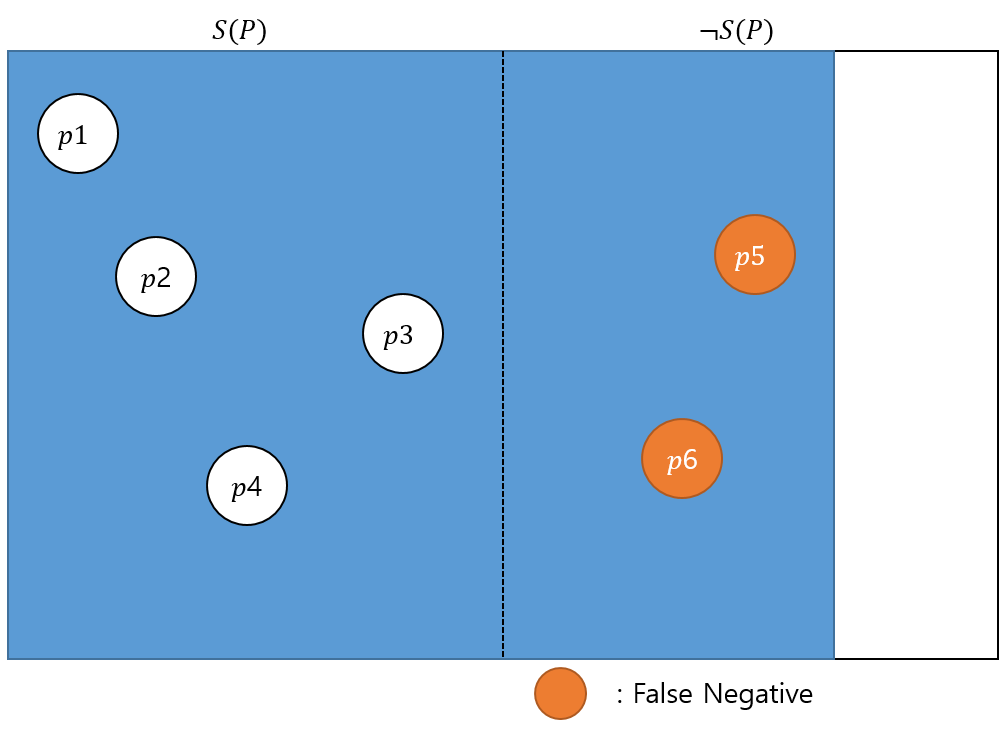
\includegraphics[width=\textwidth]{complete}
  \caption{Complete Analysis}
  \label{fig:complete}
\end{figure}

Figure \ref{fig:complete} shows a complete analysis (also the blue
area). It proves all the programs. In other words, it \textbf{wrongly
  proves} for programs $ p_5 $ and $ p_6 $ that actually do not
satisfy $ S(P) $ by accepting those programs (i.e., emitting no
alarms), thus it is \textit{unsound}. Those programs are \textbf{false
  negatives}.


The table \ref{tab:summary} shows the summary of soundness and
completeness.

\begin{table}[ht]
  \centering
  \caption{Sound \& Complete Summary}
  \label{tab:summary}

  \begin{tabular}[t]{l>{\raggedright}p{0.3\linewidth}>{\raggedright\arraybackslash}p{0.3\linewidth}}
    \hline
    & $ S(P) $ & $ \neg S(P) $ \\
    \hline
    Prove \texttt{(accept)} & \textbf{True negative} (\textsl{correct inference}) & False negative \\
    Not prove \texttt{(reject, alarm)} & False positive & \textbf{True positive} (\textsl{correct inference}) \\
    \hline
  \end{tabular}
\end{table}%



\section{Semantics of Program}
\label{sec:semantics}

Semantics of the program defines the \textbf{meaning} of the program
that is grammatically correct.

\subsection{Prerequisites}

\subsubsection{Simple Language Syntax}

\begin{math}
  \begin{array}{llll}
    a \to & \mid n & \mid x & \mid a_1 + a_2 \\
          & \mid a_1 \times a_2 & \mid a_1 - a_2 \\
    b \to & \mid \mathtt{true} & \mid \mathtt{false} & \mid a_1 = a_2  \\
          & \mid a_1 \leq a_2 & \mid \neg b & \mid b_1 \wedge b_2 \\
    c \to & \mid x := a  & \mid \mathtt{skip} & \mid c_1 ; c_2 \\
          & \mid \mathtt{if} \text{ }b \text{ }c_1\text{ }c_2 & \mid \mathtt{while} \text{ }b \text{ }c \\
  \end{array}
\end{math}

A state $ s \in State $ is a function from variables to values:
\begin{math}
  \begin{array}{rcl}
    State & : & Var \to \mathbb{Z} \\
  \end{array}
\end{math}


\subsubsection{Semantics of Arithmetic Expressions}

\begin{math}
  \begin{array}{rcl}
    \mathcal{A} & : & \mathtt{Aexp} \to State \to \mathbb{Z} \\
    \mathcal{A} \SEM{ a } & : & State \to \mathbb{Z} \\
    \mathcal{A} \SEM{ n } (s) & = & n \\
    \mathcal{A} \SEM{ x } (s) & = & s(x) \\
    \mathcal{A} \SEM{ a_1 + a_2 } (s) & = & \mathcal{A} \SEM{ a_1 } (s) + \mathcal{A} \SEM{ a_2 } (s) \\
    \mathcal{A} \SEM{ a_1 \times a_2 } (s) & = & \mathcal{A} \SEM{ a_1 } (s) \times \mathcal{A} \SEM{ a_2 } (s) \\
    \mathcal{A} \SEM{ a_1 - a_2 } (s) & = & \mathcal{A} \SEM{ a_1 } (s) - \mathcal{A} \SEM{ a_2 } (s) \\
  \end{array}
\end{math}

\subsubsection{Semantics of Boolean Expressions}

\begin{math}
  \begin{array}{rcl}
    \mathcal{B} & : & \mathtt{Bexp} \to State \to {T} \\
    {T} & = & \{ {true}, {false} \} \\
    \mathcal{B} \SEM{ b } & : & State \to {T} \\
    \mathcal{B} \SEM{ \mathtt{true} } (s) & = & {true} \\
    \mathcal{B} \SEM{ \mathtt{false} } (s) & = & {false} \\
    \mathcal{B} \SEM{ a_1 = a_2 } (s) & = & \mathcal{A} \SEM{ a_1 } (s) = \mathcal{A} \SEM{ a_2 } (s) \\
    \mathcal{B} \SEM{ a_1 \leq a_2 } (s) & = & \mathcal{A} \SEM{ a_1 } (s) \leq \mathcal{A} \SEM{ a_2 } (s) \\
    \mathcal{B} \SEM{ \neg b } (s) & = & \mathcal{B} \SEM{ b } (s) = {false} \\
    \mathcal{B} \SEM{ b_1 \wedge b_2 } (s) & = & \mathcal{B} \SEM{ b_1 } (s) \wedge \mathcal{B} \SEM{ b_2 } (s) \\
  \end{array}
\end{math}

\subsubsection{Free Variables}

A set of variables occurring in the expression.

\begin{math}
  \begin{array}{rcl}
    FV(n) & = & \emptyset \\
    FV(x) & = & \{ x \} \\
    FV(a_1 + a_2) & = & FV(a_1) \cup FV(a_2) \\
    FV(a_1 \times a_2) & = & FV(a_1) \cup FV(a_2) \\
    FV(a_1 - a_2) & = & FV(a_1) \cup FV(a_2) \\
  \end{array}
\end{math}

q\paragraph{Lemma}

Let $ s $ and $ s' $ be two states satisfying that $ s(x) = s'(x) $
for all $ x \in FV(a) $.

Then, $ \mathcal{A} \SEM{ a } (s) =\mathcal{A} \SEM{ a } (s') $ holds.

\paragraph{Lemma}

Let $ s $ and $ s' $ be two states satisrying that $ s(x) = s'(x) $
for all $ x \in FV(b) $.

Then, $ \mathcal{B} \SEM{ b } (s) = \mathcal{B} \SEM{ b } (s') $
holds.


\subsubsection{Substitution}

$ a [ y \mapsto a_0 ] $ means the arithmetic expression obtained by
replacing each occurrence of $ y $ in $a $ by $ a_0 $.

\begin{math}
  \begin{array}{rcl}
    n[y \mapsto a_0 ] & = & n \\
    x[y \mapsto a_0 ] & = & \begin{cases}
      a_0 & \mathtt{if} x = y \\
      x & \mathtt{if} x \neq y \\
    \end{cases} \\
    (a_1 + a_2)[y \mapsto a_0] & = & (a_1[y \mapsto a_0]) + (a_2[y \mapsto a_0]) \\
    (a_1 \times a_2)[y \mapsto a_0] & = & (a_1[y \mapsto a_0]) \times (a_2[y \mapsto a_0]) \\
    (a_1 - a_2)[y \mapsto a_0] & = & (a_1[y \mapsto a_0]) - (a_2[y \mapsto a_0]) \\
  \end{array}
\end{math}


\begin{math}
  (s[y \mapsto v])(x) =
  \begin{cases}
    v & \mathtt{if} x = y \\
    s(x) & \mathtt{if} x \neq y \\
  \end{cases}
\end{math}



\paragraph{Lemma}
$\mathcal{A} \SEM{ a[y \mapsto a_0] } (s) = \mathcal{A} \SEM{a} (s [ y
\mapsto \mathcal{A} \SEM{a_0} (s)]) $ for alll state s.




\subsection{Operational Semantics}

Also called as \textit{transitional} semantics.

Semantics of a program is defined by the computation steps executed on
a machine. In other words, operational semantics is concerned about
\textbf{how to execute} the program and not merly what the execution
result is.

The semantics is defined as a transition system
$ ( \mathbb{S}, \to ) $, where

\begin{itemize}
\item $ \mathbb{S} $ is the set of all \textbf{possible states}.
\item $ \to \subseteq \mathbb{S} \times \mathbb{S} $ is a
  \textbf{transition relation} between two states. Describes how the
  execution takes place.
\item $ s \in \mathbb{S} $ is a \textbf{state} of the program. It is
  either $ \pair{ S, s }$ which is a non-terminal state (i.e., the
  statement $ S $ is to be executed from the state $ s $), or $ s $
  which is a terminal state.
\end{itemize}

There are two approaches for operational semantics.  The difference
between the two are in the definitions of \textsl{transition
  relation}.

\subsubsection{Big-step}
\label{sec:big-step}

Big-step operational semantics describes how the \textbf{overall
  results} of executions are obtained.

The transition relation specified the relationship between the initial
state and the final state: $ \pair{ S, s } \to s' $

Transition relation is defined with \textbf{inference rules} of the
form:
\\

\begin{math}
\frac{ \pair{ S_1, s_1} \to s_1', ..., \pair{ S_n, s_n} \to s_n' }
{ \pair{S, s} \to s' }
\text{ if ... }
\end{math}

where

\begin{itemize}
\item $ S_1, ..., S_n $ are \textsl{statements} that consistute $ S $.
\item A rule has a number of premises and one conclusion.
\item A rule may also have a number of conditions that have to be
  fulfilled whenever the rule is applied.
\item Rules without premises are called \textbf{axioms}.
\end{itemize}

Big-step operational semantics for the while language is:


\begin{tabularx}{\textwidth}{c}
\\
$ \overline{ \pair{ x := a, s } \to s [ x \mapsto \mathcal{A}\SEM{a}(s) ] } $\\
\\
$ \overline{ \pair{ \mathtt{skip}, s} \to s } $\\
\\

$ \underline{ \pair{S_1, s} \to s' \text{   } \pair{S_2, s'} \to s''} $ \\
$ \pair{S_1;S_2, s} \to s'' $ \\
\\

\end{tabularx}


\paragraph{Semantic Function for Statements}

The \textbf{semantic function} for statements is the partial function:

\begin{math}
  \begin{array}{rcl}
    \mathcal{S}_b & : & Stm \to ( State \to State) \\
    \mathcal{S}_b \SEM{S} (s) & = &
                                    \begin{cases}
                                      s' & \mathtt{if} \pair{S, s} \to s' \\
                                      \mathbf{undef} & \mathtt{otherwise}
                                    \end{cases}

  \end{array}
\end{math}


\subsubsection{Small-step}
\label{sec:small-step}

Small-step operational semantics describes how the \textbf{individual
  steps} of the computations take place.

The individual computation steps are described by the transition
relation of the form:
\\

\begin{math}
  \pair{S, s} \implies \gamma
\end{math}

where $\gamma$ is either non-terminal state or terminal state. The
transition expresses the first step of the execution of $S$ from state
$s$.

\begin{itemize}
\item If $ \gamma = \pair{S', s'} $, non-terminal state, then the
  execution of $S$ from $s$ is not completed and the remaining
  computation continues with $\pair{S', s'}$.
\item If $ \gamma = s'$, terminal state, then the execution of $S$
  from $s$ has terminated and the final state is $s'$.
\end{itemize}

We say $\pair{S, s}$ is \textbf{stuck} if there is no $\gamma$ such
that $\pair{S, s} \implies \gamma$.

\paragraph{Semantic Function}

The semantic function $\mathcal{S}_s$ for small-step semantics is:
\begin{math}
  \begin{array}{rcl}
    \mathcal{S}_s & : & Stm \to (State \to State) \\
    \mathcal{S}_s \SEM{S} (s) & = &
                                    \begin{cases}
                                      s' & \mathtt{if} \pair{S, s} \xRightarrow{*} s' \\
                                      \mathbf{undef} & \mathtt{otherwise}
                                    \end{cases}

  \end{array}
\end{math}


\subsection{Denotational Semantics}
Also called as \textit{compositional} semantics.

Semantics of a program is defined by the semantics of the sub-parts of
the program. Thus, proving its soundness is by structural induction on
the program. For some realistic programming languages, even defining
their compositional semantics is an obstacle, due to \texttt{goto},
\texttt{exception}, or \texttt{call}.


%%% Local Variables:
%%% mode: latex
%%% TeX-master: "program-analysis"
%%% End:
